\chapter{绪论}\label{chap:introduction}
文章主要阐述微表情识别研究的意义,国内外对微表情识别相关的研究以及发展趋势,最后概述了文章的内容和结构分配。
\section{研究背景与意义}

我们人类是优秀的人脸识别专家,我们已经习惯甚至并没有意识到这一点。与其他类型的物种相比,我们人类为应对复杂的社交交互,我们的大脑已经为识别脸部信息开发了特殊的功能模块,以便我们更好地从人脸中获取更丰富的信息。

人脸是丰富的视觉信息的来源之处,我们可以从人脸中读取很多信息。如果是著名人士,我们可以立即认出他或她;如果是陌生人,我们可以对这个人的性别、年龄、种族等做出基本正确的猜测,同时如果该人脸存在表情,我们也可以大致感知他或她的情绪状态。然而尽管我们是人脸识别专家,但这并不意味着我们已经解析出了全部的人脸信息,因为仍然存在部分无法用肉眼读取的人脸信息。
神经学家保罗·麦克林(Paul Donald MacLean)于上世纪五十年代提出了“大脑三位一体”理论(The Triune Brain),他认为人类颅腔内的脑并非只有一个,而是三个,这三个脑作为人类不同进化阶段的产物,按照出现顺序依次覆盖在已有的脑层之上,如同考古遗址一样\citep{Brain1999Kazlev}。根据在进化史上出现的先后顺序,他将人脑分成“爬行动物脑”(Reptilian brain)、“古哺乳动物脑”(Paleomammalian Brain)和“新哺乳动物脑”(Neomammalian Brain)三大部分,它们分别对应人脑的脑干(Archipallium)、边缘系统(Limbic System)和新皮质(Neocortex),它们共同控制着人类的身体行为。新皮质被称作“爱说谎的大脑”,经常会因为当事人的某种需要而出现说谎的现象。语言等由新皮质大脑控制的行为是不可信的,说谎的嫌疑很大,想要得知对方内心的真实感受,就必须观察对方边缘系统所控制的表情或肢体动作。边缘系统是控制人体情感的中心,管理着人类的非语言行为表达,是分析身体语言的重点。它最大的特点是,会让人产生不加思索的本能反应,反映出一个人最真实的一面,很难被控制和掩饰。比如,听到闹轰轰的电钻声你会捂住耳朵,手被烫了会马上缩回来。所以边缘系统的行为是诚实可信的行为,是人类的思想、感觉和意图的真实反应,也是人类生存、本能的反应,它属于微反应中的除微语言以外的非语言行为反应,它包括了微动作(Micro Action)、微表情(Micro Expression),如图\ref{fig1}所示。

\begin{figure}[!htbp]
    \centering
    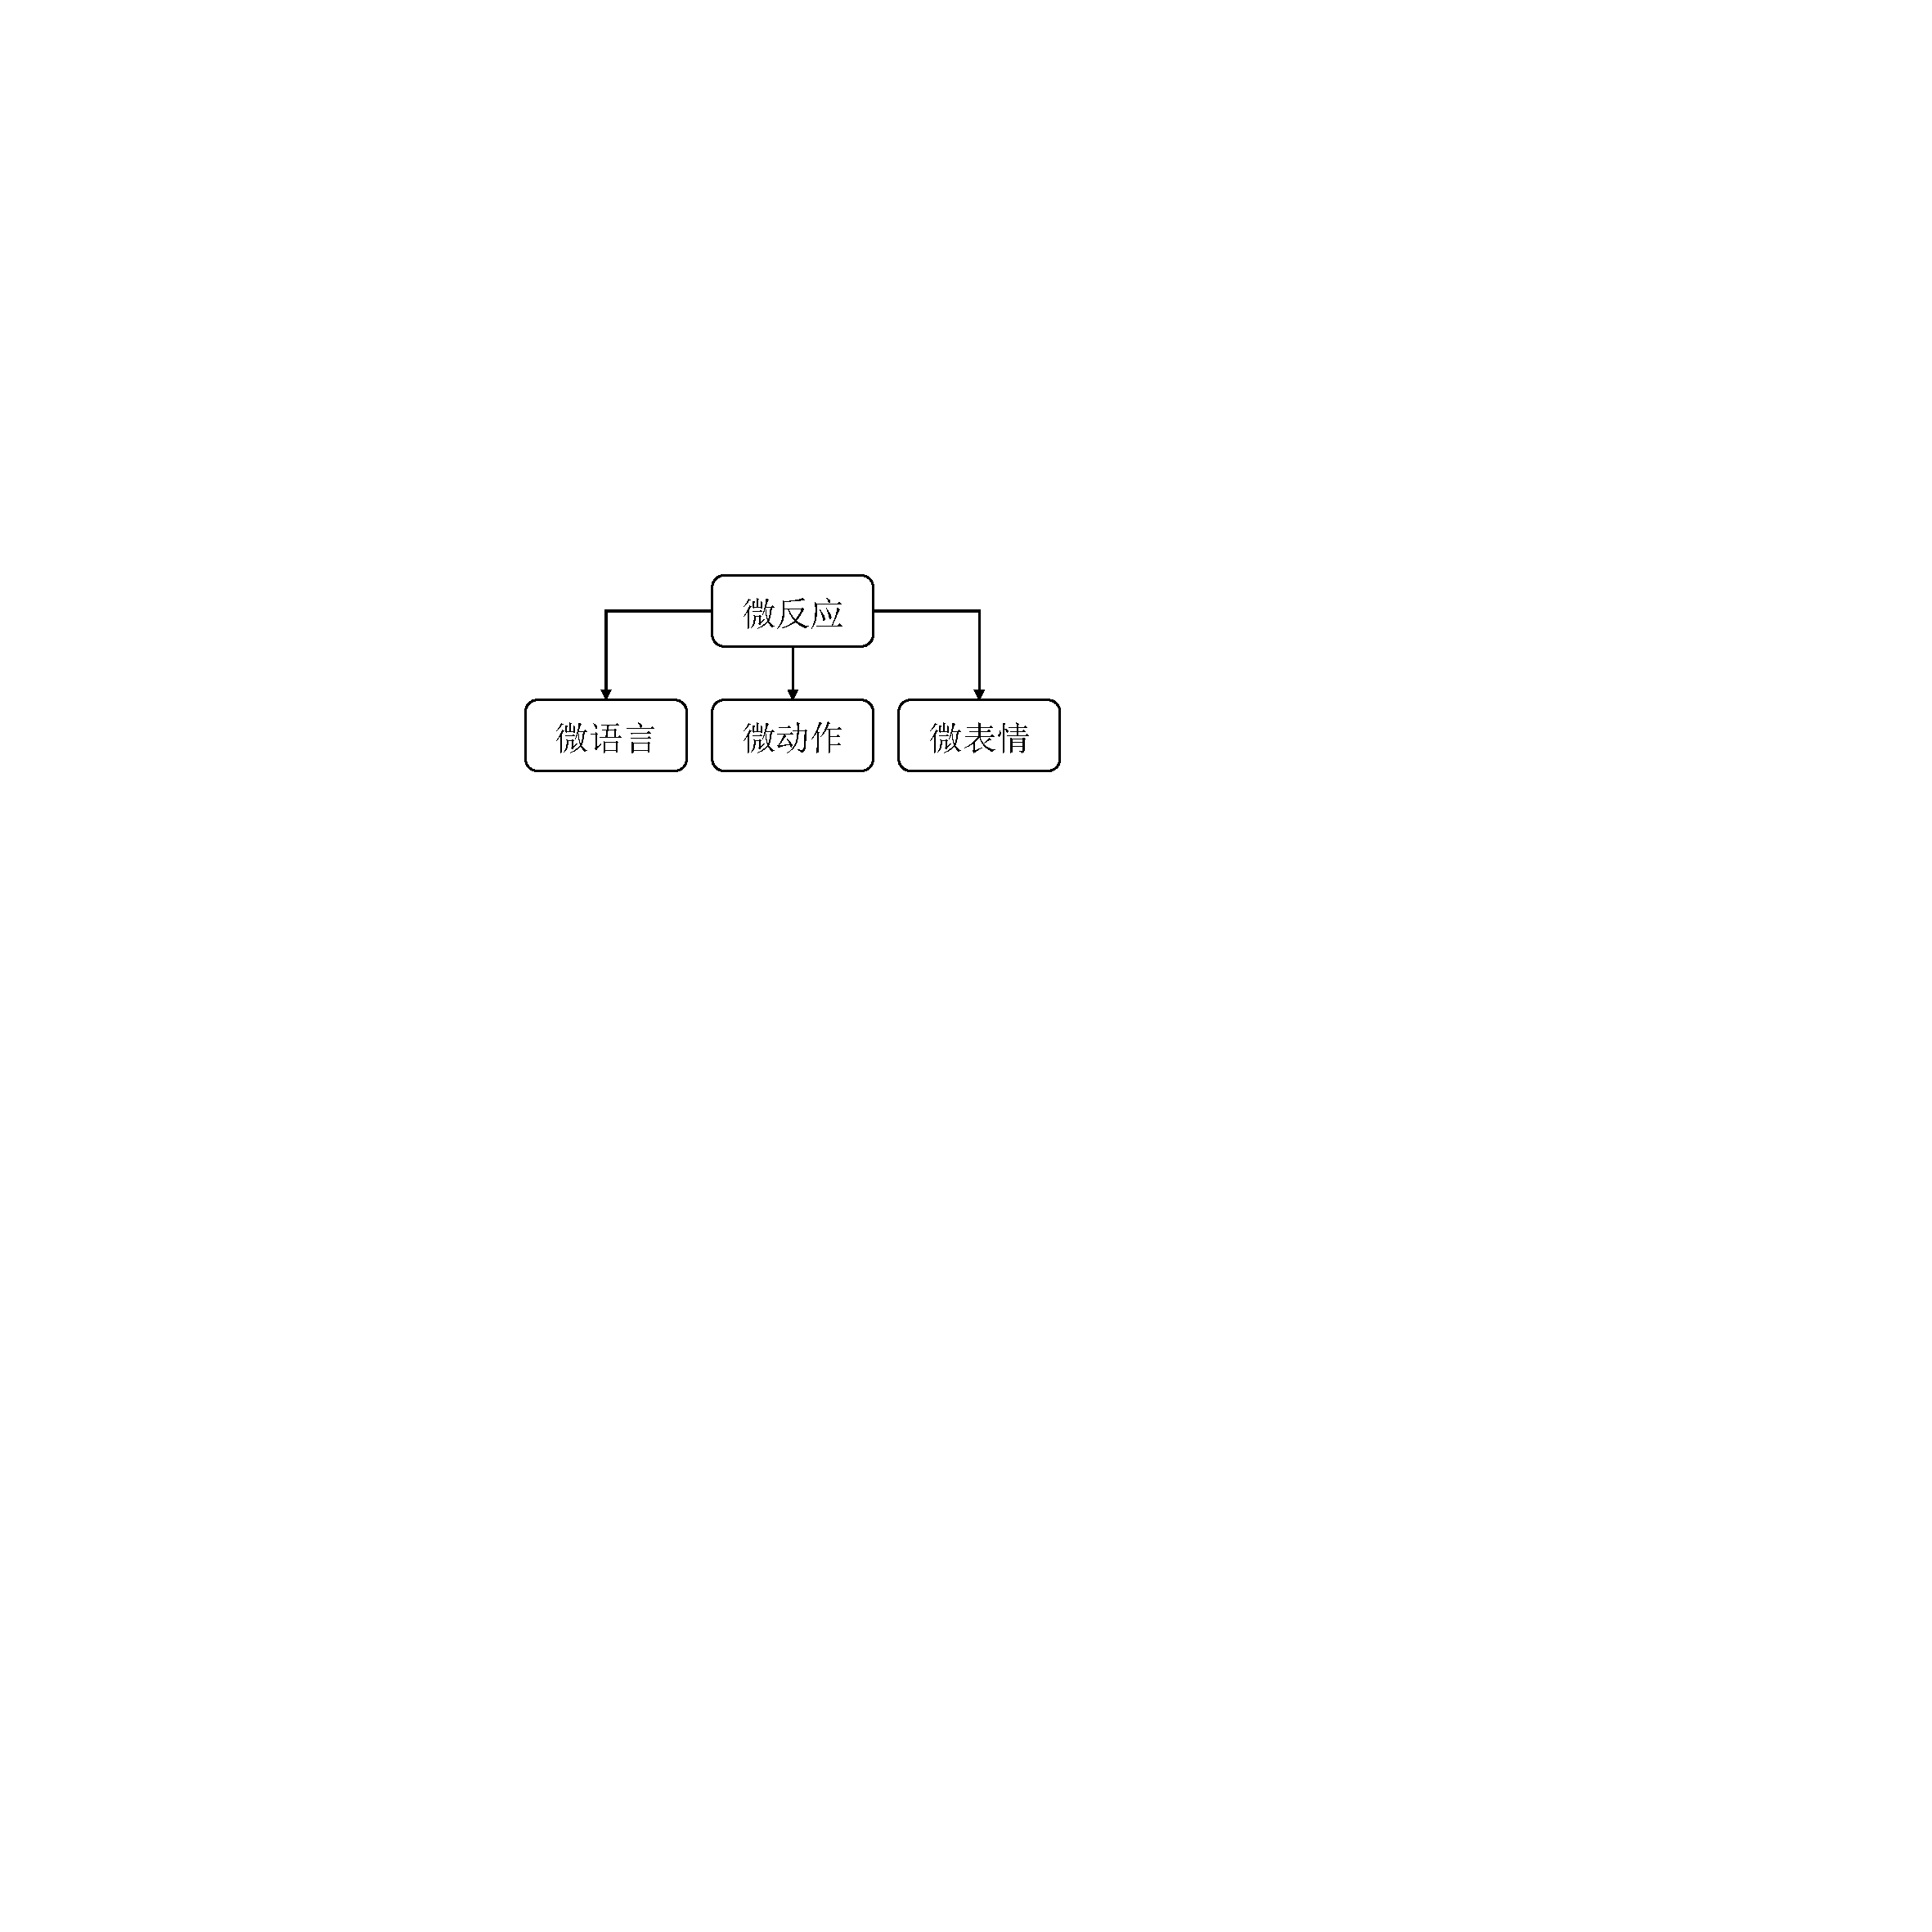
\includegraphics[width=0.40\textwidth]{img1}
    \caption{微反应的分类}   %\caption单标题注释 \caption双标题注释
    \label{fig1}
\end{figure}

美国洛杉矶大学加利福利亚分校的心理学教授艾伯特·梅拉比安(Albert Mehrabian)经过研究发现:在人类交流中,言语(谈话内容)所传递的信息量在总信息量中的份额只占7\%,声音(包括交谈时的语气,音调,音量)占38\%,剩下的55\%都来自身体语言。由此可见,身体语言能比言语传达更多有价值的信息。事实上,口头语言可以有意识地被控制,所以可能存在一定的迷惑性和欺骗性。但身体语言通常是无意识的举动,人类的主观意识很难控制身体语言行为。因此,身体语言可以最直接地暴露出人们隐藏的最真实和最深层次的想法。
身体语言是一种非言语行为,即通过身体的姿势,肢体的动作,面部的表情,眼神和目光来传递信息的一种沟通方式。简而言之,身体语言是由三部分构成的:表情语言,动作语言,空间语言。表情语言指的是通过面部肌肉运动和眼睛神态所传递出来的思想感情。动作语言则是指人类通过身体各个部位的动作或姿态来传递感情。空间语言主要指由个体与个体之间所保持的间距所形成的一种信息表达方式。
\begin{figure}[!htbp]
    \centering
    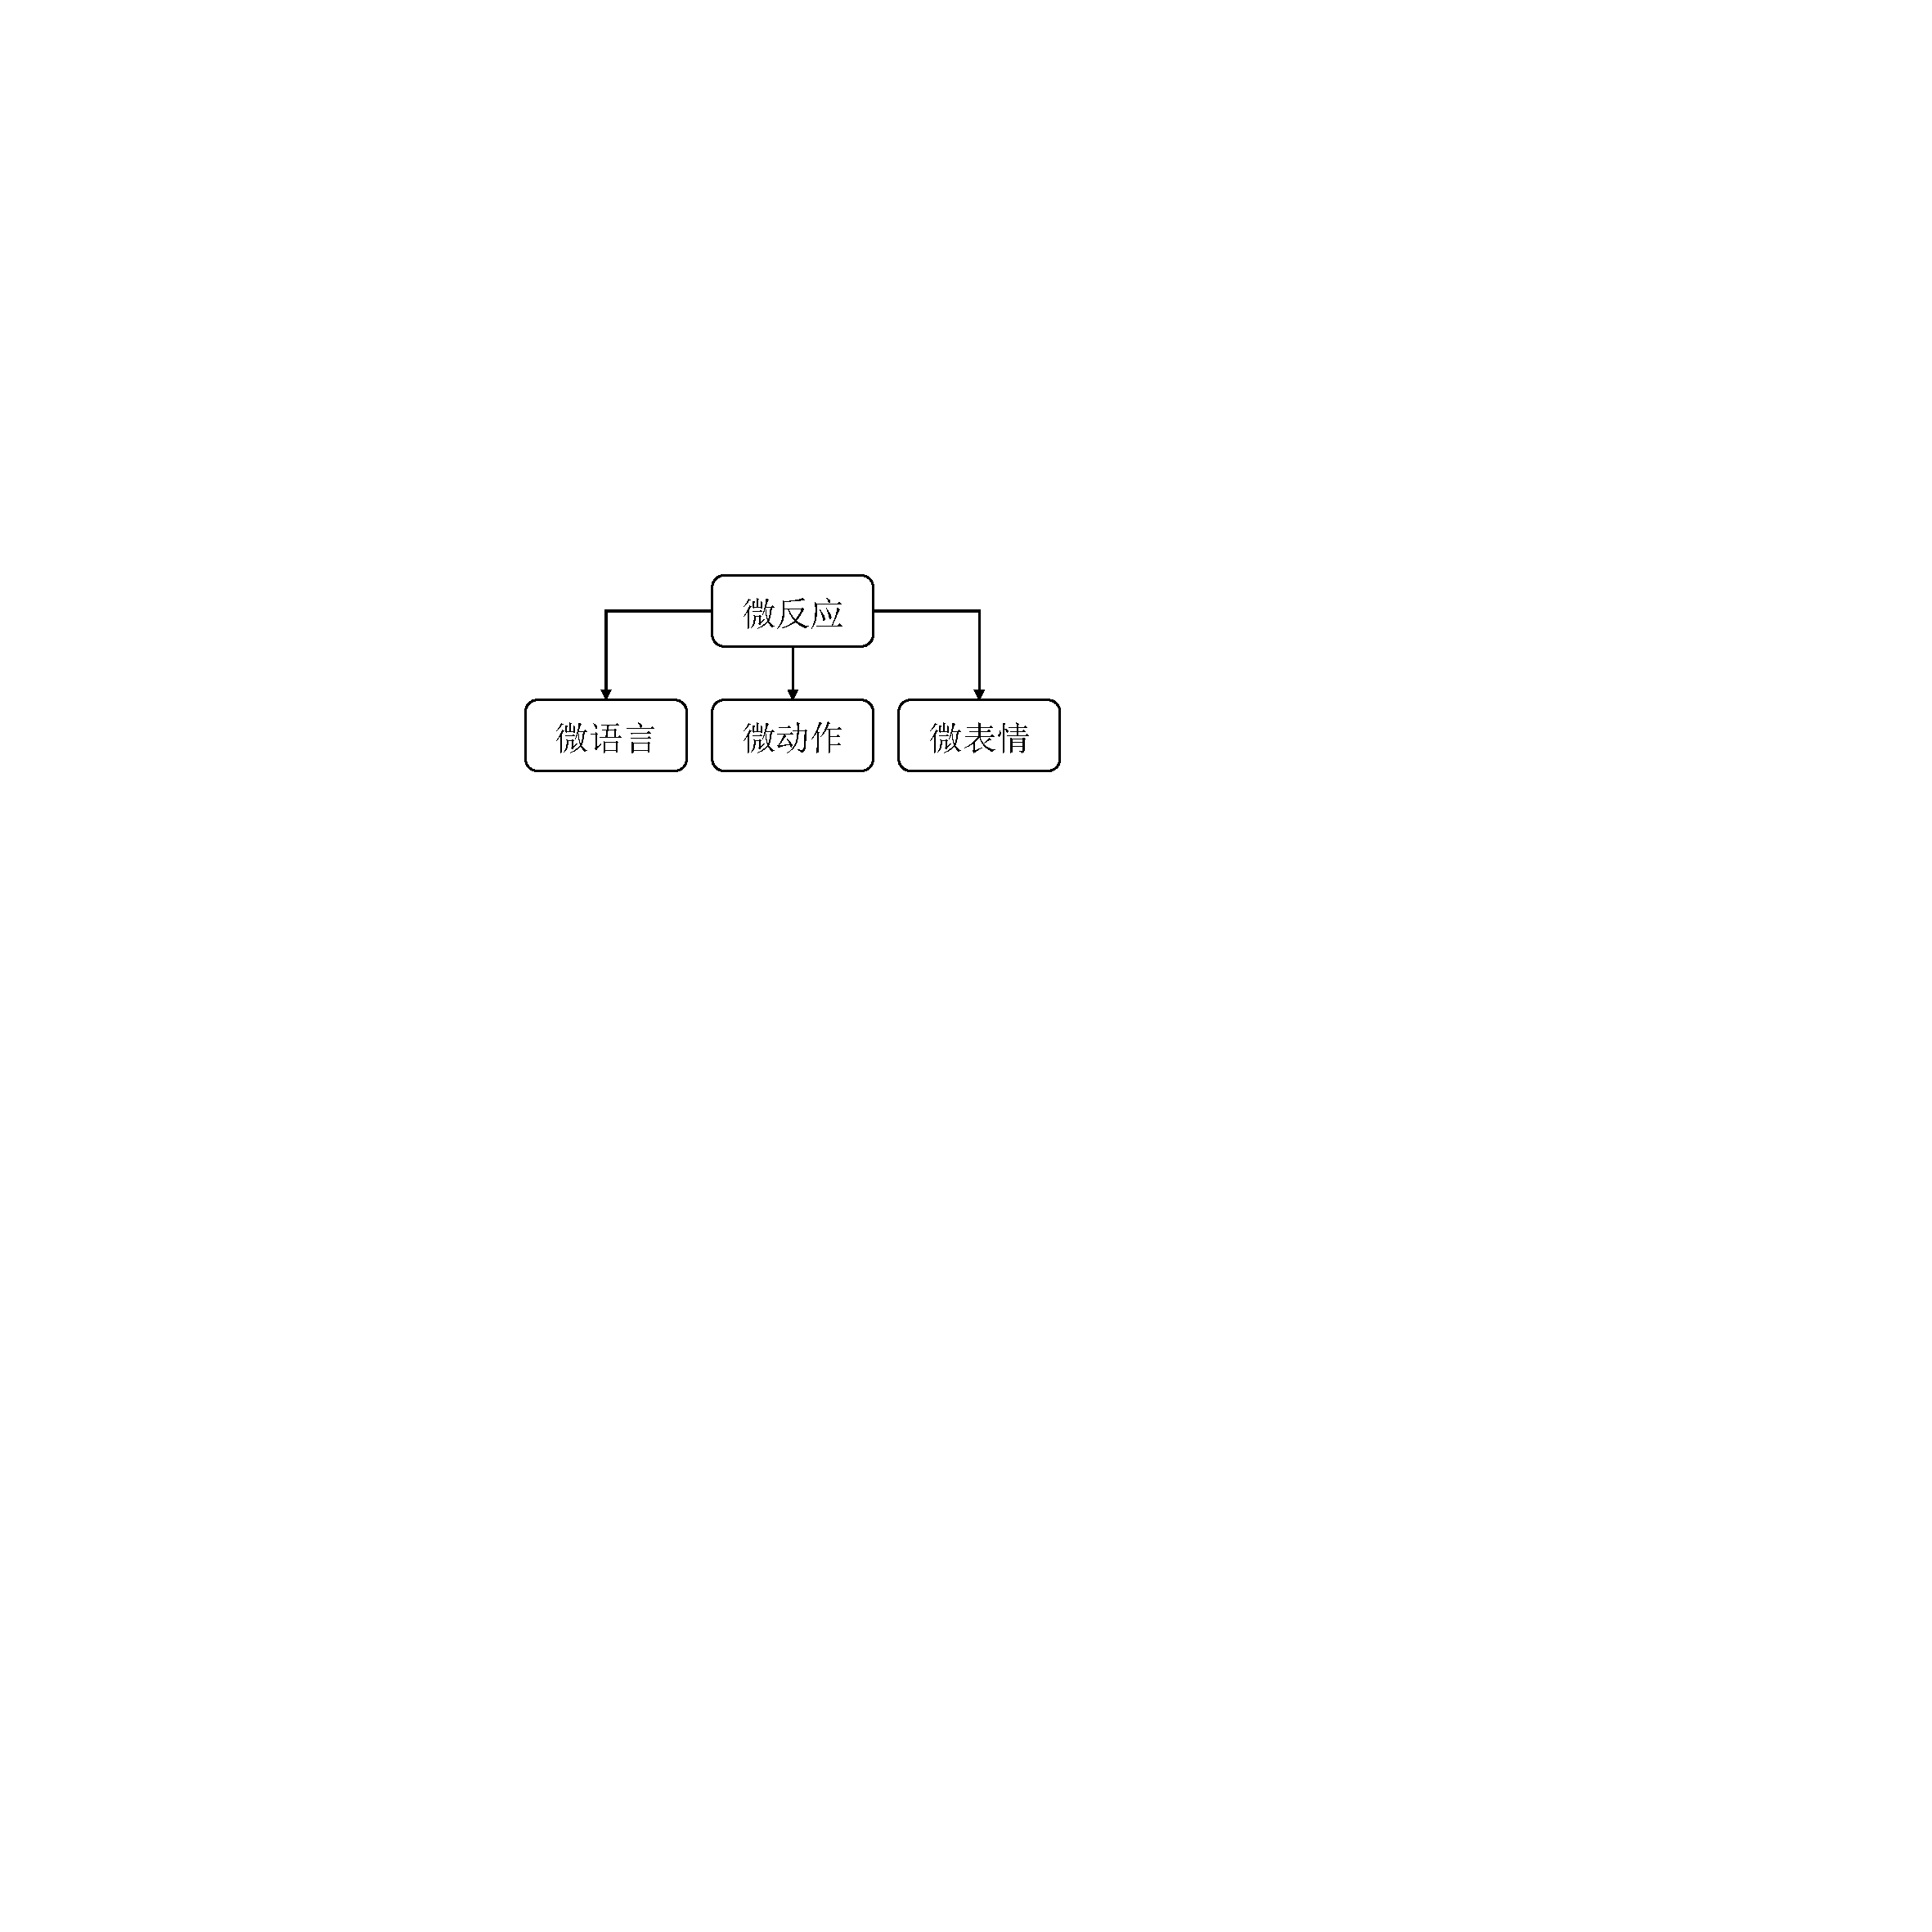
\includegraphics[width=0.40\textwidth]{img1}
    \caption{ 微反应的分类}
    \label{fig:img2}
\end{figure}

与其他感官(例如听觉和嗅觉)相比,我们的视觉认知功能在我们的大脑中更加精巧地构建。然而,我们获取视觉信息的能力仍然受到生理机制的限制。超出我们感知范围的视觉变化(在空间域中太微妙或在时域中太快)将被我们的眼睛省略。我们很难从某人的脸上看到一个ME,因为ME会短暂地发生,并且在它出现的闪光期间,所涉及的肌肉运动也太小而无法捕获。面部HR颜色的变化持续呈现在脸上,但没有人可以从脸上读出人的心率,因为颜色变化(由心脏搏动引起)对我们的眼睛来说太微妙了。但是快速和高分辨率的相机能够物理地捕捉这些微妙的视觉变化。

计算机的发明是为了帮助我们人类更好地处理信息,而人脸一直是最受欢迎的主题之一。这是一种思维方式,用于训练计算机以完成人类能够完成的任务(例如,面部检测或面部识别),并且我们训练他们更好更快地完成任务。另一方面,我们还可以训练计算机执行我们无法完成的任务,即捕获肉眼难以察觉的细微信息。我们如何训练计算机从面部视频中获取ME和HR等细微信息?这个想法导致了我论文中的所有研究工作。

微表情(Micro-expression,ME),心理学名词,心理应激微反应的一部分,是人类表达自身情感信息的重要非语言性行为。微表情从人类本能出发,在大多数情况下,不受思想的控制,无法掩饰,也不能伪装。对大部分人来说,遇到有效刺激之后的第一瞬间也会出现微表情,所以微表情总会不知不觉地暴露表情者的内在想法,从而让“谎言”有迹可寻,这是人类共有的一种特征。然而微表情总是一闪而过(最长1/2 s,最短1/25 s),所涉及的肌肉运动强度也非常微弱,甚至表情发出者和观察者都察觉不到,尤其在高风险条件下微表情出现的机率更高,被察觉的可能性也更低。

达尔文在1872年出版了《The Expression of Emotions in Man and Animals》,从此拉开了人类对面部表情的系统性研究。时至今日,人类对面部表情的研究已经非常丰富与成熟,但主要关注的是显而易见的宏观表情(Macro-expression),虽然在1966年Haggard和Isaacs首次提出了微表情现象(Micro-momentary Facial Expressions),认为微表情与自我防御机制有关,是一种被压抑的情绪,但当时并未引起人们的普遍重视。直到三年后(1969年),Ekman和Friesen在一篇文章中提出他们在观看一位有自杀倾向的精神病患者的视频时发现了微表情。视频中,患者在回答医生问题时表现的很开心,没有任何想要自杀的迹象,但之后患者向医生承认其状况并未好转,而且她在会谈时隐藏了自杀的计划。Ekman和 Friesen在逐帧慢放视频时发现了两帧和绝望有关的负面表情,只持续了1/12 s, Ekman和 Friesen将其定义为微表情,和隐藏的情感有关,这一发现奠定了微表情在临床辅助治疗上的重要地位。之后的几十年里Ekman和他的同事继续研究微表情,并引起了越来越多学术界和商业界人士的兴趣。目前在现实社会中的很多领域都已经应用到了微表情,比如国家安全、司法系统、政治选举、临床诊断、公共管理和教育领域等。Ekman的畅销书《Telling Lies》及改编的热播美剧《Lie to me》以悬疑、刑侦和鉴谎的方式介绍了微表情的部分应用。

\section{国内外研究现状}\label{sec:system}

从2005年开始,已经71岁高龄的Ekman开始对英国情报机构、美国中央情报局等各国机构进行微表情识别培训。他教辩护律师、健康专家、扑克选手,甚至对配偶心怀猜疑的人识破谎言,并且制作了网络课程。但“真相和快乐不可兼得”,Ekman坦言自己的识谎能力影响到了日常生活。他从不试图去识破周围朋友、亲戚的微表情,“去揭露每个人的微表情,揭穿每个人的谎言,这只会让自己的生活痛苦万分”。但人类对于微表情的识别能力终归是有限的,不仅要花费大量的人力和物力培训微表情识别专家,而且准确度不高,同时还伴有影响正常生活的风险。当通过摄像机和计算机系统对待分析者分析时,不仅采集到的表情真实可靠(采集中采集对象并不知情,不存在任何干扰)而且通过计算机算法可以发现细微的人类无法察觉的表情变化,并且已经有大量的实验证明计算机的识别能力确实高于人类。

早期研究中,研究人员注重于测量或训练个体的微表情识别能力。Ekman 和Friesen在1974年制作了第一个微表情识别标准测验BART(Brief Affect Recognition Test),但BART有着很大的不足——微表情孤立呈现,与现实生活中微表情的动态呈现方式不符,缺乏生态效度。1978年,Ekman发布了面部动作编码系统(Facial Action Coding System)。在这一系统中,人脸部的肌肉有43块,可以组合出1万多种表情,其中3000种具有情感意义。Ekman根据人脸解剖学特点,将其划分成若干相互独立又相互联系的运动单元(Action Unit)。分析这些运动单元的运动特征和其所控制的主要区域以及与之相关的表情,就能得出面部表情的标准运动。为了克服BART的缺陷, Matsumoto等人在2000年开发了更完善的微表情识别测量工具JACBART(Japanese and Caucasian Brief Affect Recognition Test),该测验具有很好的可信度和严密的实验过程。Ekman等人在2002年根据JACBART 开发出了一个微表情识别的训练工具METT(Micro Expression Training Tool),该训练工具有7种基本情绪的微表情,包括悲伤、恐惧、愤怒、厌恶、轻蔑、惊讶和高兴,METT 被应用在多种人群和领域,且能够成功提高受训者的微表情识别能力。
自动微表情识别系统也在如火如荼的发展中,研究者们已经开发出很多相关的算法,甚至在某些数据集的准确度可达90\%以上,但这些数据集有个明显的缺点——所有的微表情均为摆拍,这一缺点有其产生的必然性,但也严重违背了微表情的定义。为了解决这一问题,国内外的研究团队相继发表了自发微表情数据库,如中科院心理所分别在2013年和2014年发布了CASME[15]和CAMSE II两个版本的数据库,后者比前者有着更高的时空分辨率和更多的数据量,但参与者全部为蒙古利亚人种,在数据的多样性上有一定的不足;芬兰奥卢大学的CMVS团队在2013年发布了SMIC数据库,包括8名高加索人种和8名蒙古利亚人种;英国曼彻斯特城市大学在2017年发布了SAMM数据库,是目前发表最新的数据库,包括了全部人种(蒙古利亚人种、高加索人种、尼格罗人种和大洋洲人种)和均衡的性别比(见表1)。优秀的数据库提供了良好的实验基础,自动微表情识别系统的研究主要集中在微表情检测(Micro-expression Spotting)和微表情识别(Micro-expression Recognition)。
\begin{table}[!htbp]
\caption{微表情数据库比较。}
   \label{tab1}
   \centering
   \footnotesize% fontsize
   \setlength{\tabcolsep}{4pt}% column separation
   \renewcommand{\arraystretch}{1.2}%row space
   \begin{tabular}{lccccccc}
   \hline
        & SMIC-HS &  SMIC-subHS &  SMIC-NIR &  SMIC-VIS &  CASME II &  SAMM \\ \hline
微表情片段    & 164       & 71         & 71       & 71       & 247           & 159             \\
参与者      & 16        & 8          & 8        & 8        & 26            & 32              \\
分辨率      & $640\times480$   & $640\times480$    & $640\times480$  & $640\times480$  & $640\times480$       & $2040\times1088$      \\
人脸分辨率    & $190\times230$   & $190\times230$    & $190\times230$  & $190\times230$  & $280\times340$       & $400\times400$         \\
FPS      & 100       & 100        & 100      & 100      & 200           & 200             \\
性别比(F/M) & 6/10      &  2/6          &  2/6        &  2/6        & 15/11         & 16/16           \\
FACS     & NO        & NO         & NO       & NO       & YES           & YES             \\
表情类      & 3         & 3          & 3        & 3        & 5             & 7               \\
平均年龄(SD) & 26.7(N/A) &   26.7(N/A) &  26.7(N/A) & 26.7(N/A)  & 22.03(SD=1.6) & 33.24()SD=11.32 \\
人种       & 2         & 2           &  2        & 2         & 1             & 4               \\
\hline
   \end{tabular}
\end{table}

微表情的检测指在一个视频序列中自动的检测微表情发生的起始时间间隔。在论文[19]中,作者以3D梯度描述为依据,提出了一种基于3D梯度投影描述检测微表情关键帧的方法,对微表情的发现提供了一定的贡献。Wu等人提出使用Gabor滤波器构建一个自动的微表情识别系统,他们在METT训练集上达到了很高的检测性能。Shreve等人使用基于应变的光流方法检测宏观表情(Macro Expressions)和微表情(Micro Expressions)。Li等人提出将特征差异(Feature Difference)比较和峰值检测(Peak Detection)相结合检测微表情,这种方法是第一个用于真实微表情数据库检测微表情且行之有效的方法。微表情的识别是指在一段已经被确认包含微表情的序列里将微表情分为两类或更多类表情(如快乐、悲伤等)。Polikovsky等人使用3D梯度描述符来识别AU标记的微表情。Wu等人结合Gentleboost和支持向量机(Support Vector Machine,SVM)分类器来识别来自METT的合成微表情样本。Pfister等人将时间插值模型、LBP-TOP(Local Binary Patterns on Three Orthogonal Planes)特征提取和多核学习结合,是第一个基于真实的微表情数据库上提出的微表情识别方法。该方法在SMIC数据库的第一版上实现的识别准确度达71.4\%(两类分类)。Ruiz-Hernandez和Pietikäinen使用二阶高斯射流的重新参数化来生成更鲁棒的直方图,并且在SMIC数据库第一版上获得了比更好的微表情识别结果。Song等人通过从面部和身体微弱运动中学习的稀疏编码来识别情绪,他们的微表情定义更加广泛,将身体部位(脸部除外)的姿势包括在内。Wang等人从张量独立色彩空间(不是普通RGB)中提取LBP-TOP来识别微表情,其另一篇论文中将局部时空方向特征与鲁棒主成分分析(Principal Component Analysis,PCA)的稀疏部分相结合一起用于微表情识别,在CASMEII上达到了65.4\%的准确度。Li等人将低强度的微表情视频经过欧拉视频放大,在三个正交平面上利用不同的特征提取符提取特征对微表情进行识别。Huang等人将人脸的形状属性与时间和空间域上的纹理信息结合组成新的特征,同时为了提高微表情的辨别力,提出基于Laplacian的特征选择新方法,在已发表的数据库中得到了很好的识别效果。

\section{本文的研究内容}

本文简单介绍了微表情识别的基本方法和研究现状,以及其在临床诊断、国家安全、司法系统和公共管理等重要场景下不容小觑的应用价值。然而,目前的微表情研究都是基于高质量数据集的基础上展开的,例如高分辨率、大尺寸,本文结合实际应用场景提出了一种低分辨率环境下的微表情识别方法,同时分别从传统机器学习和深度学习两个角度介绍了系统框架和识别结果。文章分为六章,内容具体安排如下:

第一章:绪论。阐述了微表情研究的背景及意义,概括了国内外最新的微表情研究现状,最后对文章的整体结构做出安排;

第二章:相关工作。简单介绍了微表情的概念和微表情数据库,总结了微表情识别在传统方法和深度学习方法的进展,阐述了低分辨率微表情的识别的意义和最新进展;

第三章:基于传统方法的低分辨率环境下微表情识别的研究。主要介绍了人脸对齐与分割,其中包括对单一目标检测中主动形状模型(Active Shape Model, ASM)准确度的算法改进,图像序列的超分辨重建,三正交平面局部二值模型(Local Binary Patterns From Three Orthogonal Planes, LBP-TOP)和支持向量机分类器(Support Vector Machine, SVM);

第四章:基于深度学习的低分辨率环境下微表情识别的研究。主要介绍了伪3D残差网络(Pseudo-3D Residual Networks, P3D ResNet),数据增强以及实验分析;

第五章:低分辨率环境下微表情识别可视系统。通过对需求分析设计出系统的时序图和功能图,最后设计出功能完善的可视化系统;

第六章:总结与展望。总结全文的工作,分析不足和展望未来前景。
